\documentclass{article}
%\VignetteIndexEntry{Examples for enhanced mle code}
%\VignettePackage{bbmle}
%\VignetteDepends{aod}
%\VignetteDepends{Hmisc}
%\VignetteDepends{emdbook}
\usepackage[utf8]{inputenc} % for UTF-8/single quotes from sQuote()
\usepackage{url}
\author{Ben Bolker}
\title{Maximum likelihood estimation and analysis
  with the {\tt bbmle} package}
\newcommand{\code}[1]{{\tt #1}}
\date{\today}
\usepackage{/usr/share/R/share/texmf/Sweave}
\begin{document}
\bibliographystyle{plain}
\maketitle


The \code{bbmle} package, designed to simplify
maximum likelihood estimation and analysis in R,
extends and modifies the \code{mle} function and class
in the \code{stats4} package that comes with R by default.
\code{mle} is in turn a wrapper around the \code{optim}
function in base R.
The maximum-likelihood-estimation function and class
in \code{bbmle} are both called \code{mle2}, to avoid
confusion and conflict with the original functions in
the \code{stats4} package.  The major differences between
\code{mle} and \code{mle2} are:
\begin{itemize}
\item \code{mle2} is slightly
   more robust, with additional warnings (e.g.
  if the Hessian can't be computed by finite differences,
  \code{mle2} returns a fit with a missing Hessian rather
  than stopping with an error)
\item \code{mle2} uses a \code{data} argument to allow different
  data to be passed to the negative log-likelihood function
\item \code{mle2} has a formula interface like that
 of (e.g.) \code{gls} in the \code{nlme} package.
  For relatively simple models the formula for the
  maximum likelihood can be written in-line, rather than
  defining a negative log-likelihood function.  The formula
  interface also simplifies fitting models with
  categorical variables.  
\item \code{bbmle} defines \code{anova}, \code{AIC}, \code{AICc}, 
  and \code{BIC} methods for
  \code{mle2} objects, as well as
  \code{AICtab}, \code{BICtab}, \code{AICctab}
  functions for producing summary tables of information criteria for a 
  set of models.
\end{itemize}

Other packages with similar functionality (extending
GLMs in various ways) are \code{aod} and \code{vgam} (on CRAN), 
\code{gnlr} and \code{gnlr3} in Jim Lindsey's \code{gnlm} package
(\url{http://popgen.unimaas.nl/~jlindsey/rcode.html}).

\section{Example}

This example will use the classic data set on
\emph{Orobanche} germination from \cite{Crowder1978}
(you can also use
\code{glm(...,family="quasibinomial")} or
the \code{aod} package to analyze these data).

\subsection{Test basic fit to simulated beta-binomial data}

First, generate a single beta-binomially distributed
set of points as a simple test.

Load the \code{emdbook} package
to get functions for the beta-binomial distribution (density and random-deviate 
function --- these functions are also available
in Jim Lindsey's \code{rmutil} package).
\begin{Schunk}
\begin{Sinput}
> library(emdbook)
\end{Sinput}
\end{Schunk}

Generate random deviates from a random beta-binomial:
\begin{Schunk}
\begin{Sinput}
> set.seed(1001)
> x1 = rbetabinom(n = 1000, prob = 0.1, size = 50, theta = 10)
\end{Sinput}
\end{Schunk}

Load the package:
\begin{Schunk}
\begin{Sinput}
> library(bbmle)
\end{Sinput}
\end{Schunk}

Construct a simple negative log-likelihood function:
\begin{Schunk}
\begin{Sinput}
> mtmp <- function(prob, size, theta) {
+     -sum(dbetabinom(x1, prob, size, theta, log = TRUE))
+ }
\end{Sinput}
\end{Schunk}

Fit the model --- use \code{data} to pass the \code{size}
parameter (since it wasn't hard-coded in the \code{mtmp}
function):
\begin{Schunk}
\begin{Sinput}
> m0 <- mle2(mtmp, start = list(prob = 0.2, theta = 9), 
+     data = list(size = 50))
> m0
\end{Sinput}
\begin{Soutput}
Call:
mle2(minuslogl = mtmp, start = list(prob = 0.2, theta = 9), data = list(size = 50))

Coefficients:
      prob      theta 
 0.1030974 10.0758090 

Log-likelihood: -2723.5 
\end{Soutput}
\end{Schunk}

The \code{summary} method for \code{mle2} objects
shows the parameters; approximate standard
errors (based on quadratic approximation to the curvature at
the maximum likelihood estimate); and a test
of the parameter difference from zero based on
this standard error and on an assumption of normality.

\begin{Schunk}
\begin{Sinput}
> summary(m0)
\end{Sinput}
\begin{Soutput}
Maximum likelihood estimation

Call:
mle2(minuslogl = mtmp, start = list(prob = 0.2, theta = 9), data = list(size = 50))

Coefficients:
        Estimate Std. Error z value     Pr(z)    
prob   0.1030974  0.0031624  32.601 < 2.2e-16 ***
theta 10.0758090  0.6213189  16.217 < 2.2e-16 ***
---
Signif. codes:  0 ‘***’ 0.001 ‘**’ 0.01 ‘*’ 0.05 ‘.’ 0.1 ‘ ’ 1 

-2 log L: 5446.995 
\end{Soutput}
\end{Schunk}

Construct the likelihood profile (you can
apply \code{confint} directly to \code{m0},
but if you're going to work with the likelihood
profile (e.g. plotting, or looking for confidence
intervals at several different $\alpha$ values)
then it is more efficient to compute the profile
once):

\begin{Schunk}
\begin{Sinput}
> p0 <- profile(m0)
\end{Sinput}
\end{Schunk}

Compare the confidence interval estimates based on
inverting a spline fit to the profile (the default);
based on the quadratic approximation at the
maximum likelihood estimate; and based on
root-finding to find the exact point where the
profile crosses the critical level.

\begin{Schunk}
\begin{Sinput}
> confint(p0)
\end{Sinput}
\begin{Soutput}
           2.5 %     97.5 %
prob  0.09709228  0.1095103
theta 8.91708211 11.3559591
\end{Soutput}
\begin{Sinput}
> confint(m0, method = "quad")
\end{Sinput}
\begin{Soutput}
           2.5 %     97.5 %
prob  0.09689929  0.1092955
theta 8.85804640 11.2935716
\end{Soutput}
\begin{Sinput}
> confint(m0, method = "uniroot")
\end{Sinput}
\begin{Soutput}
           2.5 %     97.5 %
prob  0.09709185  0.1095099
theta 8.91691019 11.3559746
\end{Soutput}
\end{Schunk}

All three types of confidence limits are similar.

Plot the profiles:
\begin{Schunk}
\begin{Sinput}
> par(mfrow = c(1, 2))
> plot(p0, plot.confstr = TRUE)
\end{Sinput}
\end{Schunk}
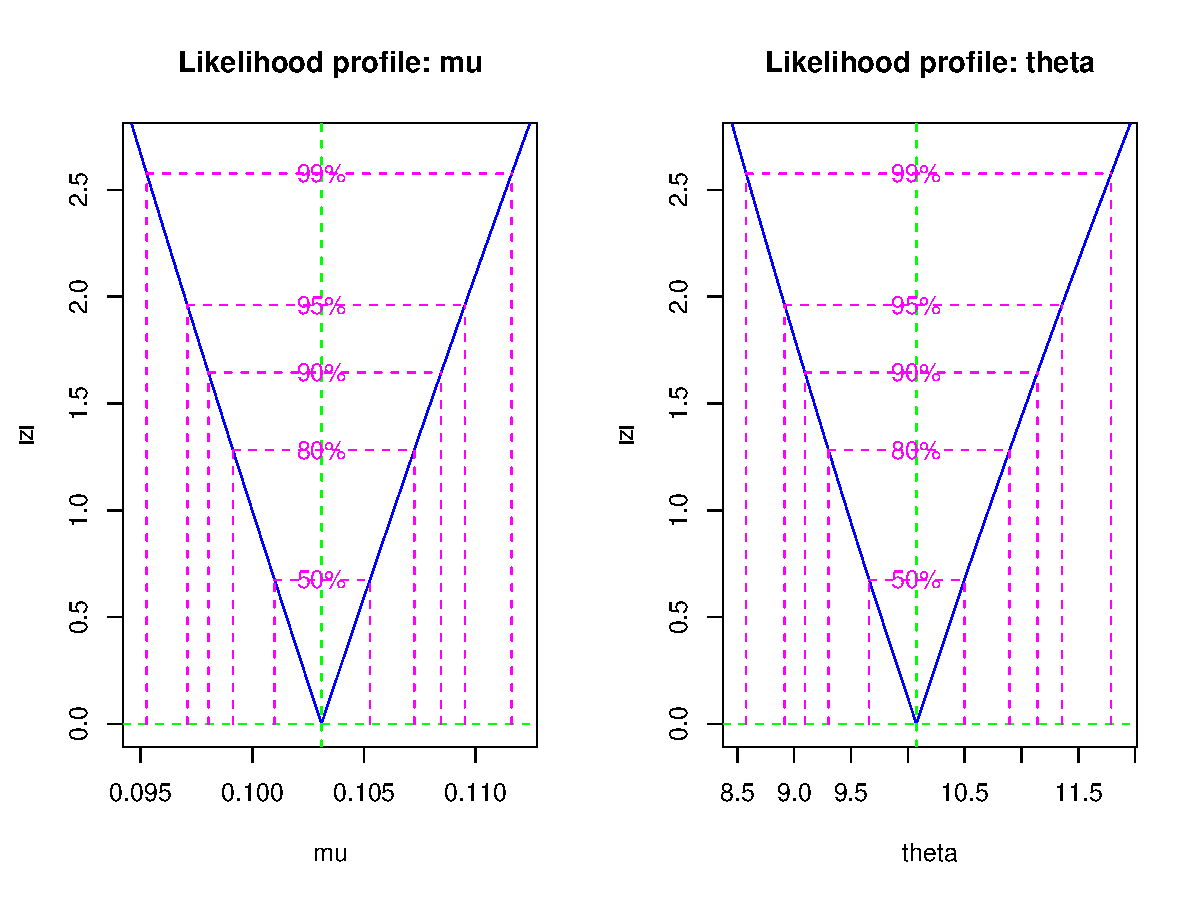
\includegraphics{mle2-010}

By default, the plot method for 
likelihood profiles displays the square root of the
the deviance
(twice the difference in negative
log-likelihood), so it will
be {\sf V}-shaped
for cases where the quadratic approximation works well
(as in this case).
(For a better visual estimate of whether the profile
is quadratic, use \code{absVal=FALSE}.)

You can also request confidence intervals
calculated using \code{uniroot}, which may be more exact when
the profile is not smooth enough to be modeled accurately
by a spline.  However, this method is
also more sensitive to numeric problems.

Instead of defining an
explicit function for \code{minuslogl}, 
we can also use the formula interface.
The formula interface assumes that
the density function given (1) has \code{x} as
its first argument (if the distribution is multivariate,
then \code{x} should be a matrix of observations)
and (2) has a \code{log} argument that will return
the log-probability or log-probability density
if \code{log=TRUE}.
\begin{Schunk}
\begin{Sinput}
> m0f <- mle2(x1 ~ dbetabinom(prob, size = 50, theta), 
+     start = list(prob = 0.2, theta = 9))
\end{Sinput}
\end{Schunk}

It's convenient to use the formula interface
to try out likelihood estimation on the
transformed parameters:
\begin{Schunk}
\begin{Sinput}
> m0cf <- mle2(x1 ~ dbetabinom(prob = plogis(lprob), size = 50, 
+     theta = exp(ltheta)), start = list(lprob = 0, ltheta = 2))
> confint(m0cf, method = "uniroot")
\end{Sinput}
\begin{Soutput}
           2.5 %    97.5 %
lprob  -2.229963 -2.095757
ltheta  2.187950  2.429744
\end{Soutput}
\begin{Sinput}
> confint(m0cf, method = "spline")
\end{Sinput}
\begin{Soutput}
           2.5 %    97.5 %
lprob  -2.229963 -2.095756
ltheta  2.187948  2.429742
\end{Soutput}
\end{Schunk}

In this case the answers from \code{uniroot}
and \code{spline} (default) methods barely
differ.

\subsection{Using real data}
Get data from Crowder 1978 \cite{Crowder1978},
as incorporated in the \code{aod} package:
\begin{Schunk}
\begin{Sinput}
> library(aod)
\end{Sinput}
\begin{Soutput}
Package aod, version 1.1-22 
\end{Soutput}
\begin{Sinput}
> data(orob1)
\end{Sinput}
\end{Schunk}

Now construct a negative log-likelihood
function that differentiates among groups:
\begin{Schunk}
\begin{Sinput}
> ML1 <- function(prob1, prob2, prob3, theta, x) {
+     prob <- c(prob1, prob2, prob3)[as.numeric(x$dilution)]
+     size <- x$n
+     -sum(dbetabinom(x$y, prob, size, theta, log = TRUE))
+ }
\end{Sinput}
\end{Schunk}

Results from \cite{Crowder1978}:
% latex.default(crowder.results, file = "", table.env = FALSE,      title = "model") 
%
\begin{center}
 \begin{tabular}{lrrrrrrrr}\hline\hline
\multicolumn{1}{l}{model}&
\multicolumn{1}{c}{prob1}&
\multicolumn{1}{c}{prob2}&
\multicolumn{1}{c}{prob3}&
\multicolumn{1}{c}{theta}&
\multicolumn{1}{c}{sd.prob1}&
\multicolumn{1}{c}{sd.prob2}&
\multicolumn{1}{c}{sd.prob3}&
\multicolumn{1}{c}{NLL}
\\ \hline
prop diffs&$0.132$&$0.871$&$0.839$&$78.424$&$0.027$&$0.028$&$0.032$&$-34.991$\\
full model&$$&$$&$$&$$&$$&$$&$$&$-34.829$\\
homog model&$$&$$&$$&$$&$$&$$&$$&$-56.258$\\
\hline
\end{tabular}

\end{center}                            
\begin{Schunk}
\begin{Sinput}
> m1 <- mle2(ML1, start = list(prob1 = 0.5, prob2 = 0.5, 
+     prob3 = 0.5, theta = 1), data = list(x = orob1))
> m1
\end{Sinput}
\begin{Soutput}
Call:
mle2(minuslogl = ML1, start = list(prob1 = 0.5, prob2 = 0.5, 
    prob3 = 0.5, theta = 1), data = list(x = orob1))

Coefficients:
     prob1      prob2      prob3      theta 
 0.1318287  0.8706204  0.8382700 73.6958477 

Log-likelihood: -34.99 

Warning: optimization did not converge (code 1)
\end{Soutput}
\end{Schunk}

The result warns us that the optimization has not
converged; we also don't match
Crowder's results for $\theta$ exactly.
We can fix this by setting \code{parscale} appropriately.

\begin{Schunk}
\begin{Sinput}
> m2 <- mle2(ML1, start = as.list(coef(m1)), control = list(parscale = coef(m1)), 
+     data = list(x = orob1))
\end{Sinput}
\end{Schunk}

\begin{Schunk}
\begin{Sinput}
> m2
\end{Sinput}
\begin{Soutput}
Call:
mle2(minuslogl = ML1, start = as.list(coef(m1)), data = list(x = orob1), 
    control = list(parscale = coef(m1)))

Coefficients:
     prob1      prob2      prob3      theta 
 0.1322123  0.8708914  0.8393195 78.4227872 

Log-likelihood: -34.99 
\end{Soutput}
\end{Schunk}

Calculate likelihood profile:
\begin{Schunk}
\begin{Sinput}
> p2 <- profile(m2)
\end{Sinput}
\end{Schunk}

Get the curvature-based parameter standard
deviations (which Crowder used
rather than computing likelihood profiles):
\begin{Schunk}
\begin{Sinput}
> round(sqrt(diag(vcov(m2))), 3)
\end{Sinput}
\begin{Soutput}
 prob1  prob2  prob3  theta 
 0.028  0.029  0.032 74.238 
\end{Soutput}
\end{Schunk}
We are slightly off Crowder's numbers --- rounding
error?

Crowder also defines a variance (overdispersion) parameter
$\sigma^2=1/(1+\theta)$.
\begin{Schunk}
\begin{Sinput}
> sqrt(1/(1 + coef(m2)["theta"]))
\end{Sinput}
\begin{Soutput}
    theta 
0.1122089 
\end{Soutput}
\end{Schunk}

Using the delta method to get the standard deviation of
$\sigma$:
\begin{Schunk}
\begin{Sinput}
> sqrt(deltavar(sqrt(1/(1 + theta)), meanval = coef(m2)["theta"], 
+     vars = "theta", Sigma = vcov(m2)[4, 4]))
\end{Sinput}
\begin{Soutput}
[1] 0.05244163
\end{Soutput}
\end{Schunk}

Another way to fit in terms of $\sigma$ rather than $\theta$
is to compute $\theta=1/\sigma^2-1$ on the fly in a
formula:

\begin{Schunk}
\begin{Sinput}
> m2b <- mle2(y ~ dbetabinom(prob, size = n, theta = 1/sigma^2 - 
+     1), data = orob1, parameters = list(prob ~ dilution, 
+     sigma ~ 1), start = list(prob = 0.5, sigma = 0.1))
> round(sqrt(diag(vcov(m2b))), 3)["sigma"]
\end{Sinput}
\begin{Soutput}
sigma 
0.052 
\end{Soutput}
\begin{Sinput}
> p2b <- profile(m2b)
\end{Sinput}
\end{Schunk}

As might be expected since the standard deviation
of $\sigma$ is large, the quadratic approximation is
poor:

\begin{Schunk}
\begin{Sinput}
> r1 <- rbind(confint(p2)["theta", ], confint(m2, method = "quad")["theta", 
+     ])
> rownames(r1) <- c("spline", "quad")
> r1
\end{Sinput}
\begin{Soutput}
           2.5 %   97.5 %
spline  19.81826       NA
quad   -67.08021 223.9258
\end{Soutput}
\end{Schunk}

Plot the profile:
\begin{Schunk}
\begin{Sinput}
> plot(p2, which = "theta", plot.confstr = TRUE)
\end{Sinput}
\end{Schunk}
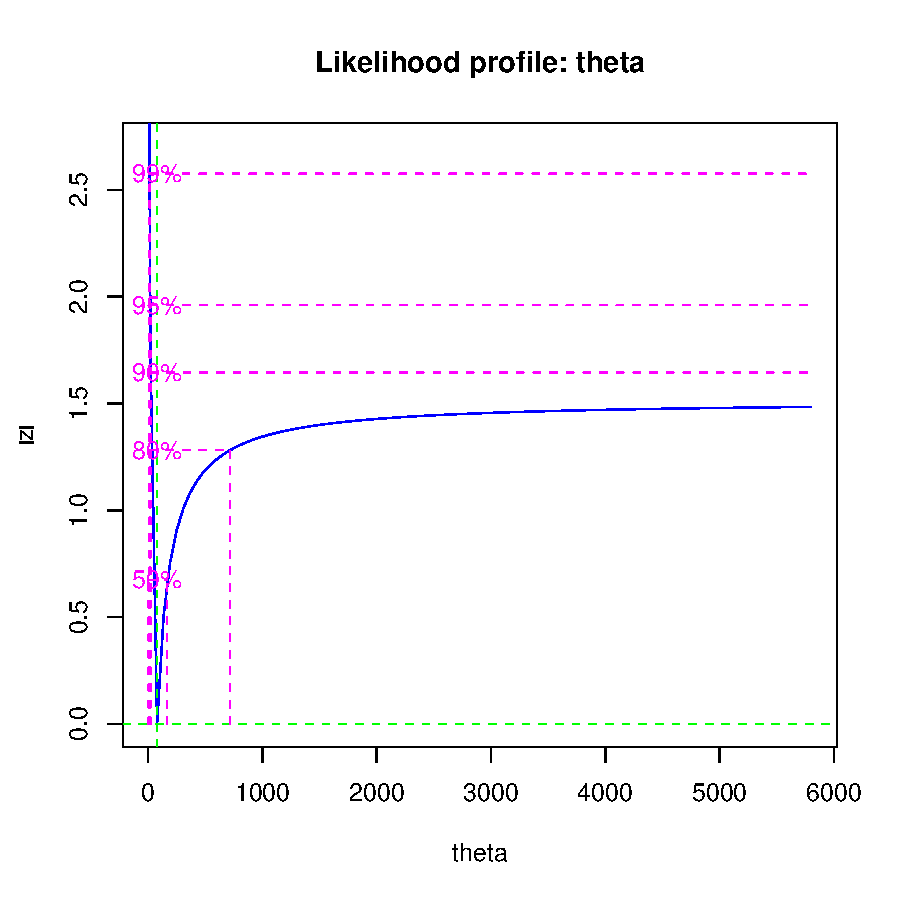
\includegraphics{mle2-025}

What does the profile for $\sigma$ look like?
\begin{Schunk}
\begin{Sinput}
> plot(p2b, which = "sigma", plot.confstr = TRUE, show.points = TRUE)
\end{Sinput}
\end{Schunk}
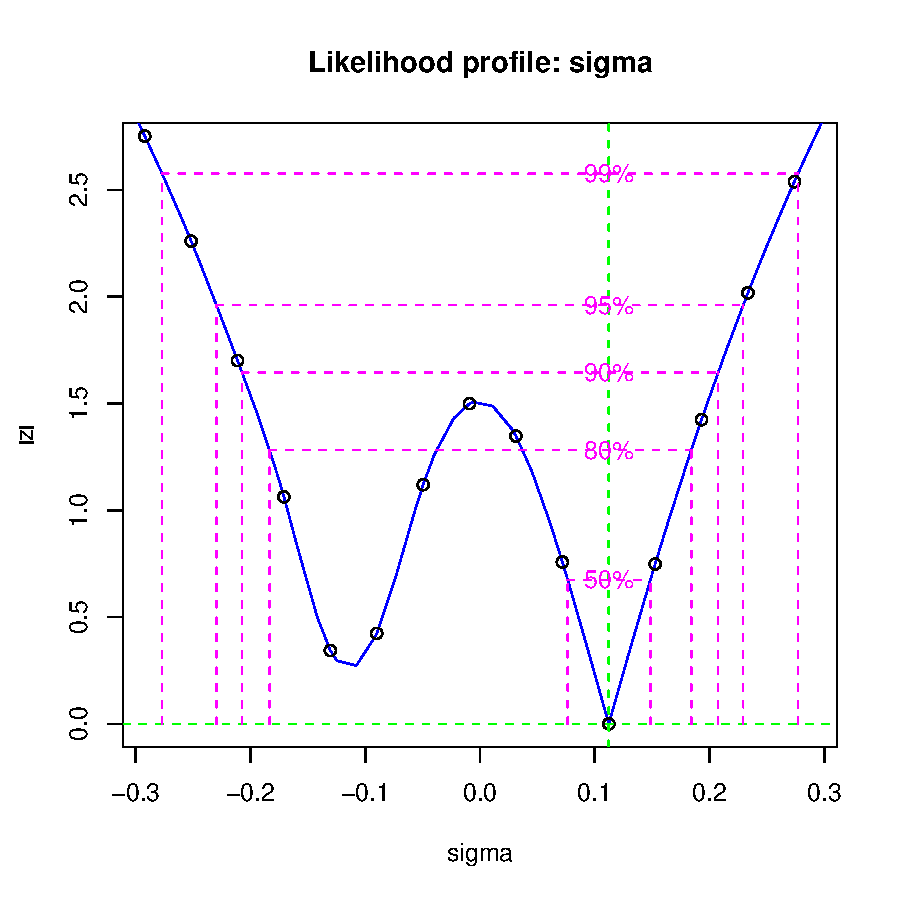
\includegraphics{mle2-026}

Now fit a homogeneous model:
\begin{Schunk}
\begin{Sinput}
> ml0 <- function(prob, theta, x) {
+     size <- x$n
+     -sum(dbetabinom(x$y, prob, size, theta, log = TRUE))
+ }
> m0 <- mle2(ml0, start = list(prob = 0.5, theta = 100), 
+     data = list(x = orob1))
\end{Sinput}
\end{Schunk}

The log-likelihood matches Crowder's result:
\begin{Schunk}
\begin{Sinput}
> logLik(m0)
\end{Sinput}
\begin{Soutput}
'log Lik.' -56.25774 (df=2)
\end{Soutput}
\end{Schunk}

It's easier to 
use the formula interface
to specify all three of the models
fitted by Crowder (homogeneous, probabilities differing
by group, probabilities and overdispersion differing
by group):

\begin{Schunk}
\begin{Sinput}
> m0f <- mle2(y ~ dbetabinom(prob, size = n, theta), parameters = list(prob ~ 
+     1, theta ~ 1), data = orob1, start = list(prob = 0.5, 
+     theta = 100))
> m2f <- mle2(y ~ dbetabinom(prob, size = n, theta), parameters = list(prob ~ 
+     dilution, theta ~ 1), data = orob1, start = list(prob = 0.5, 
+     theta = 78.424))
> m3f <- mle2(y ~ dbetabinom(prob, size = n, theta), parameters = list(prob ~ 
+     dilution, theta ~ dilution), data = orob1, start = list(prob = 0.5, 
+     theta = 78.424))
\end{Sinput}
\end{Schunk}

\code{anova} runs a likelihood ratio test on nested
models:
\begin{Schunk}
\begin{Sinput}
> anova(m0f, m2f, m3f)
\end{Sinput}
\begin{Soutput}
Likelihood Ratio Tests
Model 1: m0f, y~dbetabinom(prob,size=n,theta): prob~1, theta~1
Model 2: m2f, y~dbetabinom(prob,size=n,theta): prob~dilution, theta~1
Model 3: m3f, y~dbetabinom(prob,size=n,theta): prob~dilution,
          theta~dilution
  Tot Df Deviance   Chisq Df Pr(>Chisq)    
1      2  112.515                          
2      4   69.981 42.5341  2  5.805e-10 ***
3      6   69.981  0.0008  2     0.9996    
---
Signif. codes:  0 ‘***’ 0.001 ‘**’ 0.01 ‘*’ 0.05 ‘.’ 0.1 ‘ ’ 1 
\end{Soutput}
\end{Schunk}

The various \code{ICtab} commands produce tables of
information criteria, optionally sorted and
with model weights.
\begin{Schunk}
\begin{Sinput}
> AICtab(m0f, m2f, m3f, weights = TRUE, delta = TRUE, sort = TRUE)
\end{Sinput}
\begin{Soutput}
    AIC   df dAIC  weight
m2f  78.0 4    0.0 0.881 
m3f  82.0 6    4.0 0.119 
m0f 116.5 2   38.5 <0.001
\end{Soutput}
\begin{Sinput}
> BICtab(m0f, m2f, m3f, delta = TRUE, nobs = nrow(orob1), 
+     sort = TRUE, weights = TRUE)
\end{Sinput}
\begin{Soutput}
    BIC   df dBIC  weight
m2f  81.1 4    0.0 0.941 
m3f  86.6 6    5.5 0.059 
m0f 118.1 2   37.0 <0.001
\end{Soutput}
\begin{Sinput}
> AICctab(m0f, m2f, m3f, delta = TRUE, nobs = nrow(orob1), 
+     sort = TRUE, weights = TRUE)
\end{Sinput}
\begin{Soutput}
    AICc  df dAICc weight
m2f  81.6 4    0.0 0.992 
m3f  91.3 6    9.7 0.008 
m0f 117.4 2   35.8 <0.001
\end{Soutput}
\end{Schunk}

\section*{Additions/enhancements/differences from \code{stats4::mle}}
\begin{itemize}
\item{\code{anova} method}
\item{warnings on convergence failure}
\item{more robust to non-positive-definite Hessian;
  can also specify \code{skip.hessian} to skip Hessian
  computation when it is problematic}
\item{when profiling fails because better value is
    found, report new values}
\item{can take named vectors as well as lists as
    starting parameter vectors}
\item{added \code{AICc}, \code{BIC} definitions,
    \code{ICtab} functions}
\item{added \code{"uniroot"} and \code{"quad"}
    options to \code{confint}}
\item{more options for colors and line types etc etc.
The old arguments are:
\begin{Schunk}
\begin{Sinput}
> function(x, levels, conf = c(99, 95, 90, 80, 50)/100, 
+     nseg = 50, absVal = TRUE, ...) {
+ }
\end{Sinput}
\end{Schunk}
The new one is:
\begin{Schunk}
\begin{Sinput}
> function(x, levels, which = 1:p, conf = c(99, 95, 90, 
+     80, 50)/100, nseg = 50, plot.confstr = FALSE, confstr = NULL, 
+     absVal = TRUE, add = FALSE, col.minval = "green", 
+     lty.minval = 2, col.conf = "magenta", lty.conf = 2, 
+     col.prof = "blue", lty.prof = 1, xlabs = nm, ylab = "score", 
+     show.points = FALSE, main, xlim, ylim, ...) {
+ }
\end{Sinput}
\end{Schunk}
\code{which} selects (by character vector or numbers)
which parameters to plot: \code{nseg} does nothing
(even in the old version); \code{plot.confstr} turns on
the labels for the confidence levels; \code{confstr} gives
the labels; \code{add} specifies whether to add the
profile to an existing plot; \code{col} and \code{lty}
options specify the colors and line types for
horizontal and vertical lines marking the minimum
and confidence vals and the profile curve; \code{xlabs}
gives a vector of x labels; \code{ylab} gives the y label;
\code{show.points} specifies whether to show the raw points
computed.
}
\item{\code{mle.options()}}
\item{\code{data} argument}
\item{handling of names in argument lists}
\item{can use alternative optimizers (\code{nlminb}, \code{constrOptim})}
\end{itemize}

\section*{Bugs, wishes, to do}
\begin{itemize}
\item \textbf{BUG}: \code{mle2} fits that are obtained within a function
  can't be used for subsequent profiles etc. (environment issue)
\item \textbf{WISH}: \code{subset} and \code{predict}
\item minor \textbf{WISH}: 
  better methods for extracting \code{nobs} information
  when possible (e.g. with formula interface)
\item \textbf{WISH}: better documentation, especially for S4 methods
\item \textbf{WISH}: variable-length chunks in argument list
\item \textbf{WISH}: limited automatic differentiation
    (add capability for common distributions)
\end{itemize}

\bibliography{mle2}
\end{document}
